\chapter{Re\c{t}ele neuronale convolu\c{t}ionale}

Re\c{t}elele neuronale convolu\c{t}ionale  sunt foarte similare cu re\c{t}elele neuronale obi\c{s}nuite din capitolul anterior, ele sunt formate din neuroni care \^{i}nva\c{t}\u{a} \^{i}nt\u{a}riri \c{s}i bias-uri care s\u{a} \^{i}ndeplineasc\u{a} o anumit\u{a} sarcin\u{a}. Fiecare neuron prime\c{s}te date de intrare de la neuronii de pe nivelul inferiro lor, efectuaz\u{a} o opera\c{t}ie de multiplicare \^{i}ntre \^{i}nt\u{a}rir \c{s}i datele de intrare, adun\u{a} bias-ul la rezultatul ob\c{t}inut \^{i}n urma multiplic\u{a}rii iar dup\u{a} de cele mai multe ori aplic\u{a} o func\c{t}ie de activare, iar la final dup\u{a} ultimul nivel aplic\u{a}o func\c{t}ie de cost care s\u{a} determine c\^{a}t de aproape este re\c{t}eaua neuronal\u{a} de adevar \c{s}i dup\u{a} se aplic\u{a} propagarea \^{i}napoi pentru a actualiza \^{i}nt\u{a}ririle \c{s}i bias-ruile de pe fiecare nivel astfle \^{i}nc\^{a}t ca la urmatorul pas de \^{i}nv\u{a}\c{t}are a re\c{t}elei neuroanle aceasta s\u{a} ob\c{t}in\u{a} un rezultat mai mic de la func\c{t}ia de cost.

La prima vedere re\c{t}elele neuronale convolu\c{t}ionale seamana foarte mult cu re\c{t}elele neuronale obi\c{s}nuite, un lucru adevarat, \^{i}ns\u{a} exista unele diferen\c{t}e \^{i}ntre ele. Rec\c{t}elele neuronale convolutionale pleac\u{a} de la prezum\c{t}ia c\u{a} datele de intrare de pe primul nivel sunt imagini, fa\c{t}\u{a} de re\c{t}elele neuronale obi\c{s}nuite unde datele de intrare de pe primul nivel sunt ni\c{s}te vectori, din aceast\u{a} cauz\u{a} re\c{t}elele neuronale convolu\c{t}ionale se pot folosii de unele propiet\u{a}\c{t}i ale imaginilor asfel \^{i}nc\^{a}t acestea s\u{a} fiu mai eficiente in sarcini ce implica imaginile \c{s}i mai u\c{s}or de antrenat deoarece au nevoie de mai pu\c{t}ini parametrii dec\^{a}t ar avea nevoie o re\c{t}ea nuronale obi\c{s}nuit\u{a} \^{i}n \^{i}ndeplinirea aceleia\c{s}i sarcini.

\section{Arhitectura unei re\c{t}ele neuronale convolutionale}

Re\c{t}elele neuronale convolutionale folosesc trei idei de baz\i{a} : local receptive fields, shared weights \c{s}i pooling.

\par

Local receptive fields : in loc sa mai luam fiecare valoare a unui pixel separat \c{s}i s\u{a} o introducem intr-un neuron de pe un nivel intermediar ( hidden layer ) ca dat\u{a} de intrare putem s\u{a} grup\u{a}m pixelii in blocuri de pixeli \c{s}i s\u{a} \^{i}i trimitem grupa\c{t}i la un neuron de pe primul nivel intermediar ( hidden layer ).   Cum se observ\u{a} \c{s}i \^{i}n imaginea de mai jos, un grup de 5 x 5 pixeli este trimis grupat c\u{a}tre un singru neuron de pe primul nivel intermediar.

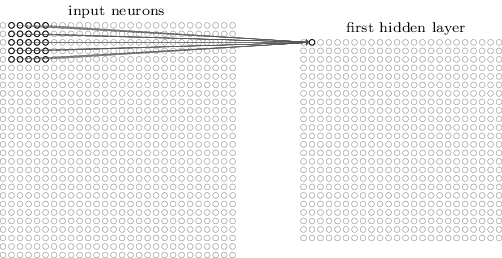
\includegraphics[width=300]{conv.png}

Fieacre bloc de pixeli are c\^{a}te o greutate ( weights ), iar neuronul de pe nivelul intermediar care prime\c{s}te acest bloc de pixeli ca dat\u{a} de intreare are un bias / un trashold.

\par

Dac\u{a} spargem o imagine de 28 x 28 pixeli in blocuri de 5 x 5 pixeli \c{s}i ne mi\c{s}c\u{a}m cu un pixel la dreapta sau in jos pentru fiecare bloc de pixeli pe care vrem s\u{a} \^{i}l extragem, atunci pe primul nivel intermediar vom avea 24 x 24 de valori.

\par

Shared weights and biases : se va folosii acela\c{s} weights si bias pentru fiecare neuron de pe primul nivel intermediar.

\par

Pooling layers: nivelul de pooling se pune intre doua nivele convolutionale pentru a se reduce cantitatea de informa\c{t}ie care se duce c\u{a}tre urm\u{a}torul nivel convolutional. Cel mai folosit tip de pooling este max-pooling care prime\c{s}te ca date de intrare valorile rezultate de la precedentul nivel convolutional \c{s}i le las\u{a} s\u{a} treac\u{a} doar pe cel cu valoarea cea mai mare catre urmatorul nivel convolutional ( vede\c{t}i imaginea de mai jos ), astfle c\u{a} acest nivel ne ajut\u{a} s\u{a} reducem cantitatea de date \c{s}i s\u{a} sc\u{a}p\u{a}m de datele nerelevante dintr-o re\c{t}ea convolutional\u{a}.

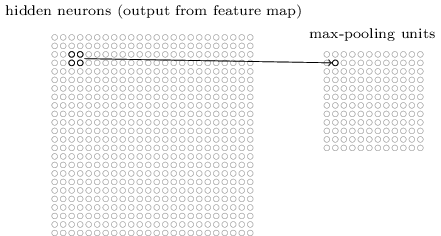
\includegraphics[width=300]{pool.png}

Cum se observ\u{a} \^{i}n imaginea de mai sus, nivelul de max-pooling prime\c{s}te patru valori de pe nivelul preceden \c{s}i las\u{a} o singur\u{a} valoarea s\u{a} treac\u{a} mai departe.